% Báo cáo phần Thành viên 3: Related Work & Experiments cho MoVE-KD.
% Biên dịch: xelatex tv3_report.tex (2 lần) trong thư mục report/. Hình lấy từ ../images/.
\documentclass[11pt,a4paper]{article}

\usepackage{fontspec}
\setmainfont{texgyretermes}[
  Extension = .otf,
  UprightFont = *-regular,
  BoldFont = *-bold,
  ItalicFont = *-italic,
  BoldItalicFont = *-bolditalic]
\setmonofont{lmmono10-regular.otf}[Scale=0.95]

\usepackage[margin=2.4cm]{geometry}
\usepackage{amsmath}
\usepackage{graphicx}
\usepackage{booktabs}
\usepackage{tabularx}
\usepackage{array}
\usepackage{float}
\usepackage[font=small,labelfont=bf]{caption}
\usepackage{subcaption}
\usepackage{xcolor}
\usepackage{listings}
\usepackage{enumitem}
\usepackage[colorlinks=true,linkcolor=blue!60!black,citecolor=blue!60!black,urlcolor=blue!60!black]{hyperref}

\graphicspath{{../images/}}
\setlist{itemsep=2pt,topsep=4pt}
\renewcommand{\arraystretch}{1.15}
\newcolumntype{R}{>{\raggedleft\arraybackslash}X}
\usepackage{xurl}
% \path (gói url) cho phép ngắt dòng trong tên file/lệnh dài
\DeclareRobustCommand{\code}[1]{\path{#1}}
\emergencystretch=2em
\newcommand{\best}[1]{\textbf{#1}}

\lstset{basicstyle=\ttfamily\small,columns=fullflexible,frame=single,
  backgroundcolor=\color{gray!6},rulecolor=\color{gray!40},breaklines=true,
  keepspaces=true,showstringspaces=false}

\renewcommand{\figurename}{Hình}
\renewcommand{\tablename}{Bảng}
\renewcommand{\contentsname}{Mục lục}
\renewcommand{\refname}{Tài liệu tham khảo}
\renewcommand{\abstractname}{Tóm tắt}

\title{\textbf{MoVE-KD: Related Work \& Experiments}\\[4pt]
\large Báo cáo phần Thành viên 3 -- Thực nghiệm, Benchmark \& Code Execution}
\author{Nhóm đồ án Thị giác máy tính}
\date{Tháng 11/2026}

\begin{document}
\maketitle

\begin{abstract}
Báo cáo này trình bày các công trình liên quan và phần thực nghiệm của MoVE-KD \cite{movekd}, phương pháp chưng cất nhiều vision encoder (CLIP, EVA-02, ConvNeXt, SAM) vào một CLIP ViT-L/14-336 duy nhất trong LLaVA-1.5. Ngoài việc tổng hợp kết quả và ablation của paper, chúng tôi tự chạy lại toàn bộ 4 benchmark chấm được tại máy (POPE, MME, TextVQA, ScienceQA) trên 1$\times$RTX~3090. Checkpoint công bố tái lập đúng số liệu paper (lệch $\le 0.2$ điểm). Tuy nhiên, khi chạy baseline LLaVA-1.5-7B trong cùng điều kiện, ScienceQA của baseline cao hơn con số paper dùng 2.7 điểm, khiến mức tăng của MoVE-KD trên benchmark này giảm từ $+3.0$ xuống $+0.4$. Chúng tôi cũng trực quan hoá [CLS] attention và routing của MoLE, đồng thời chạy thử pipeline huấn luyện Stage~1 với đủ 4 teacher. Trong quá trình này, chúng tôi phát hiện và sửa một bug khiến code huấn luyện công bố không chạy được.
\end{abstract}

\tableofcontents
\newpage

% =====================================================================
\section{Related Work}

\subsection{Vision-Language Models}

\paragraph{Kiến trúc encoder $\rightarrow$ connector $\rightarrow$ LLM.} Hướng phổ biến để xây VLM là ``gắn mắt'' cho LLM. Một vision encoder đã tiền huấn luyện (thường là CLIP, vốn đã căn chỉnh với ngôn ngữ) trích đặc trưng ảnh, một khối kết nối đưa đặc trưng vào không gian embedding của LLM, rồi cả hệ được huấn luyện trên dữ liệu ảnh--văn bản. Các mô hình khác nhau chủ yếu ở khối kết nối (Bảng~\ref{tab:vlm}).

\begin{table}[H]
\centering
\caption{Cách nối đặc trưng ảnh vào LLM ở một số VLM tiêu biểu.}
\label{tab:vlm}
\begin{tabularx}{\linewidth}{@{}lX@{}}
\toprule
Mô hình & Cách nối ảnh vào LLM \\
\midrule
Flamingo \cite{flamingo} & Chèn các lớp \emph{gated cross-attention} vào giữa LLM đóng băng \\
BLIP-2 / InstructBLIP \cite{blip2} & \emph{Q-Former}: tập query học được nén đặc trưng ảnh thành ít token \\
Qwen-VL \cite{qwenvl} & Adapter cross-attention một lớp, nén về số token cố định \\
\textbf{LLaVA / LLaVA-1.5} \cite{llava} & Chiếu \emph{mọi} patch token bằng MLP 2 lớp; huấn luyện 2 giai đoạn (LCS-558K rồi mix665k) \\
LLaVA-NeXT & Thêm \emph{AnyRes}: cắt ảnh độ phân giải cao thành nhiều ô rồi nối chuỗi token \\
\bottomrule
\end{tabularx}
\end{table}

MoVE-KD được xây trên LLaVA-1.5 (và thử thêm trên LLaVA-NeXT), nên mọi so sánh trong paper đều lấy chính LLaVA làm baseline, với cùng dữ liệu và cùng quy trình huấn luyện.

\paragraph{Tăng cường vision encoder.} Vì chất lượng encoder giới hạn năng lực của cả VLM, nhiều nghiên cứu tìm cách làm phần ``nhìn'' mạnh hơn. Hướng thứ nhất là \emph{tăng độ phân giải hoặc số nhánh}: S$^2$ \cite{s2} chạy cùng một encoder ở nhiều tỉ lệ ảnh, còn LLaVA-NeXT cắt ảnh thành nhiều ô. Hướng thứ hai là \emph{ghép nhiều encoder}: Mini-Gemini \cite{minigemini} thêm một encoder ConvNeXt độ phân giải cao; SPHINX \cite{sphinx} trộn embedding của nhiều encoder; Eagle \cite{eagle} khảo sát có hệ thống việc kết hợp CLIP, ConvNeXt, EVA-02, Pix2Struct, SAM và cho thấy chỉ cần nối kênh đã hiệu quả; Cambrian-1 \cite{cambrian} dùng \emph{Spatial Vision Aggregator}. MoVE-KD chọn bộ teacher theo kết quả của Eagle, và phần lớn code teacher trong repo cũng được mượn từ Eagle.

\paragraph{Hạn chế mà MoVE-KD nhắm tới.} Các hướng trên đều \emph{tăng chi phí suy luận}: ảnh lớn hơn, nhiều token hơn, hoặc phải chạy nhiều encoder cho mỗi ảnh. MoVE-KD đi theo hướng ngược lại: nhiều encoder chỉ tham gia lúc huấn luyện (làm teacher), còn lúc suy luận vẫn chỉ có \textbf{một} CLIP ViT-L/14-336 cùng một lượng nhỏ tham số LoRA.

\subsection{Knowledge Distillation}

\paragraph{KD kinh điển.} Hinton và cộng sự \cite{hinton} cho student học phân phối mềm của teacher (``dark knowledge''). FitNets \cite{fitnets} mở rộng sang \emph{feature distillation}, ép đặc trưng trung gian của student khớp với teacher qua một lớp chiếu. MoVE-KD thuộc nhánh feature distillation, với loss MSE giữa token của student và token của teacher đã qua adapter.

\paragraph{KD cho vision encoder.} DINOv2 \cite{dinov2} dùng self-distillation; Feature Distillation \cite{fd} chưng cất từ một teacher CLIP. Cả hai chỉ có \textbf{một} teacher. Công trình gần nhất là AM-RADIO \cite{radio}: chưng cất đồng thời CLIP, DINOv2 và SAM vào một ViT trên DataComp-1B (khoảng 1,4 tỉ cặp ảnh--văn bản), rồi thay encoder đó vào LLaVA. Theia và UNIC \cite{theia} cũng chưng cất đa teacher nhưng \emph{độc lập}, bên ngoài VLM. Điểm khác của MoVE-KD là \textbf{chưng cất ngay trong khung VLM}: loss KD cộng thẳng vào loss sinh văn bản và dùng chính dữ liệu của LLaVA.

\paragraph{KD với nhiều teacher.} You và cộng sự \cite{multiteacher} huấn luyện student dưới giám sát của nhiều teacher; OneS \cite{ones} gom tri thức từ nhiều expert vào một mô hình dày đặc; LLaVA-MoD \cite{llavamod} chưng cất kiểu MoE nhưng ở phía LLM. Theo các tác giả, MoVE-KD là công trình đầu tiên chưng cất \textbf{nhiều vision encoder} để cải thiện VLM.

\paragraph{Trọng số cho token và teacher.} Ý tưởng ``không phải token nào cũng đáng chưng cất như nhau'' đã có ở \emph{Masked Distillation with Receptive Tokens} \cite{mdrt}. ``Vision Transformers Need Registers'' \cite{registers} phát hiện các token ``artifact'' có attention cao ở vùng nền. MoVE-KD dùng [CLS] attention của CLIP làm trọng số token và cố ý giữ các artifact token.

\subsection{Mixture-of-Experts và LoRA}

MoE \cite{moe} dùng router chỉ kích hoạt một phần expert cho mỗi token, tăng dung lượng mà không tăng chi phí tương ứng. Trong VLM, MoE-LLaVA và Uni-MoE \cite{moellava} đưa MoE vào \textbf{LLM}. LoRA \cite{lora} học phần bù hạng thấp $\Delta W = BA$. Kết hợp hai ý tưởng cho ra \emph{mixture of LoRA experts} (LoRAMoE, MoLE \cite{mole}). MoVE-KD áp dụng MoLE vào \textbf{vision encoder} với mục đích khác: để các expert LoRA ``chia việc'' khi student học đồng thời từ nhiều teacher có không gian đặc trưng mâu thuẫn.

\subsection{Vị trí của MoVE-KD}

\begin{table}[H]
\centering
\caption{So sánh MoVE-KD với các hướng gần nhất.}
\begin{tabularx}{\linewidth}{@{}lXXX@{}}
\toprule
 & Encoder lúc suy luận & Thêm dữ liệu? & Chưng cất trong VLM? \\
\midrule
Eagle / Cambrian-1 / Mini-Gemini & Nhiều encoder & Tuỳ & Không (ghép trực tiếp) \\
AM-RADIO & 1 encoder & Có (DataComp-1B) & Không (chưng cất trước) \\
\textbf{MoVE-KD} & \textbf{1 CLIP + MoLE} & \textbf{Không} & \textbf{Có} \\
\bottomrule
\end{tabularx}
\end{table}

% =====================================================================
\section{Thiết lập thực nghiệm}

\paragraph{Mô hình.} Khung chính là LLaVA-1.5 với LLM Vicuna-7B/13B; paper thử thêm MobileLLaMA-1.4B và LLaVA-NeXT 7B/13B. Student là CLIP ViT-L/14-336 được thay các FFN bằng MoLE gồm 3 expert, rank 32.

\paragraph{Teacher.} MoVE-KD-v1.0 dùng CLIP, EVA-02-L, ConvNeXt-XXL (\code{--encoder_teachers clip eva convnext}); v1.1 thêm \textbf{SAM-L}. Hai script \code{pretrain-v1.0.sh} và \code{pretrain-v1.1.sh} chỉ khác nhau ở dòng này và ở thư mục output, nên so sánh v1.0 với v1.1 chính là ablation ``thêm teacher SAM''.

\paragraph{Dữ liệu và huấn luyện.} Pre-train dùng LCS-558K, fine-tune dùng mix665k của LLaVA-1.5; paper \textbf{không thêm dữ liệu}. Cả hai giai đoạn tối ưu
\begin{equation}
\mathcal{L}_{\text{total}} = \mathcal{L}_{\text{text}} + \lambda_{\text{bal}}\,\mathcal{L}_{\text{balance}} + \lambda_{\text{kd}}\,\mathcal{L}_{\text{kd}},
\end{equation}
với cấu hình ở Bảng~\ref{tab:hparams}. Paper huấn luyện trên 16$\times$A800; các thông số còn lại giữ như LLaVA (bf16, ZeRO-2, cosine schedule, warmup 3\%, độ dài tối đa 2048).

\begin{table}[H]
\centering
\caption{Hai giai đoạn huấn luyện và hyper-parameter, đối chiếu giữa paper và \code{scripts/move-kd/*.sh}.}
\label{tab:hparams}
\begin{tabularx}{\linewidth}{@{}lXX@{}}
\toprule
 & Stage 1 -- Pre-train & Stage 2 -- Fine-tune \\
\midrule
Tham số được học & MoLE, encoder adapter, projector & Toàn bộ, trừ teacher \\
Learning rate / batch mỗi GPU & $10^{-3}$ / 16 & $2\times10^{-5}$ / 8 \\
\midrule
$\lambda_{\text{kd}}$ (\code{--kd_w}) & \multicolumn{2}{l}{0.5} \\
Trọng số teacher CLIP (\code{--kd_memory_w}) & \multicolumn{2}{l}{0.8} \\
Số expert / rank LoRA & \multicolumn{2}{l}{3 / 32} \\
$\lambda_{\text{bal}}$ (\code{--moe_encoder_balance_w}) & \multicolumn{2}{l}{0.01 (paper không nêu)} \\
Token weight / teacher weight & \multicolumn{2}{l}{bật} \\
\bottomrule
\end{tabularx}
\end{table}

\paragraph{Benchmark.} Paper dùng 8 benchmark (Bảng~\ref{tab:bench}). VQAv2, VizWiz và MMB phải nộp lên server, nên phần tự chạy lại chỉ làm 4 benchmark chấm được tại máy: POPE, MME, TextVQA, SQA.

\begin{table}[H]
\centering
\caption{Tám benchmark dùng trong paper.}
\label{tab:bench}
\small
\begin{tabularx}{\linewidth}{@{}lXlll@{}}
\toprule
Benchmark & Năng lực đánh giá & Quy mô & Metric & Chấm \\
\midrule
VQAv2 & VQA tổng quát & test-dev, $\sim$107K & VQA acc. & Server \\
GQA & Suy luận cấu trúc, quan hệ không gian & $\sim$12,6K & Acc. & Local \\
TextVQA & Đọc chữ trong ảnh & val, 5000 & VQA acc. & Local \\
VizWiz & Ảnh người khiếm thị chụp & test, 8000 & VQA acc. & Server \\
POPE & Ảo giác đối tượng (yes/no) & 3 split, 8910 & F1 TB & Local \\
SQA & ScienceQA trắc nghiệm có ảnh & test-IMG, 2017 & Acc. & Local \\
MME & Perception (10 tác vụ con) & 2374 & Tổng điểm & Local \\
MMB & MMBench đa năng lực & dev & CircularEval & Server \\
\bottomrule
\end{tabularx}
\end{table}

% =====================================================================
\section{Kết quả chính}

Bảng~\ref{tab:main} là các dòng LLaVA-1.5 trong Table~1 của paper.

\begin{table}[H]
\centering
\caption{Kết quả chính (Table 1 của paper). In đậm: tốt nhất trong từng khối.}
\label{tab:main}
\small
\setlength{\tabcolsep}{4pt}
\begin{tabular}{@{}llrrrrrrrr@{}}
\toprule
Phương pháp & LLM & VQAv2 & GQA & TextVQA & VizWiz & POPE & SQA & MME & MMB \\
\midrule
LLaVA-1.5 & MobileLLaMA-1.4B & 71.5 & 55.4 & 42.6 & 28.6 & 84.3 & 56.0 & 1145.7 & 47.0 \\
+ MoVE-KD-v1.0 & MobileLLaMA-1.4B & 72.9 & 56.6 & 43.4 & \best{32.1} & 84.8 & 56.1 & 1182.3 & 47.4 \\
+ MoVE-KD-v1.1 & MobileLLaMA-1.4B & \best{73.8} & \best{57.7} & \best{44.3} & 29.3 & \best{86.1} & \best{57.3} & \best{1188.4} & \best{48.8} \\
\midrule
LLaVA-1.5 & Vicuna-7B & 78.5 & 62.0 & 58.2 & 50.0 & 85.9 & 66.8 & 1510.7 & 64.3 \\
+ RADIO & Vicuna-7B & 76.3 & 63.0 & 56.3 & -- & 86.2 & -- & -- & -- \\
+ MoVE-KD-v1.0 & Vicuna-7B & 79.5 & 63.2 & 58.3 & 52.3 & \best{86.9} & 69.3 & \best{1524.5} & 66.3 \\
+ MoVE-KD-v1.1 & Vicuna-7B & \best{79.9} & \best{63.9} & \best{59.6} & \best{52.7} & 86.3 & \best{69.8} & 1509.1 & \best{67.4} \\
\midrule
LLaVA-1.5 & Vicuna-13B & 80.0 & 63.3 & \best{61.3} & 53.6 & 85.9 & 71.6 & 1531.3 & 67.7 \\
+ MoVE-KD-v1.0 & Vicuna-13B & 80.6 & \best{64.2} & 59.7 & 55.7 & 85.7 & \best{73.2} & 1568.1 & \best{70.2} \\
+ MoVE-KD-v1.1 & Vicuna-13B & \best{80.8} & 63.9 & 61.1 & \best{57.5} & \best{86.3} & 71.8 & \best{1568.3} & 69.7 \\
\bottomrule
\end{tabular}
\end{table}

\begin{figure}[H]
\centering
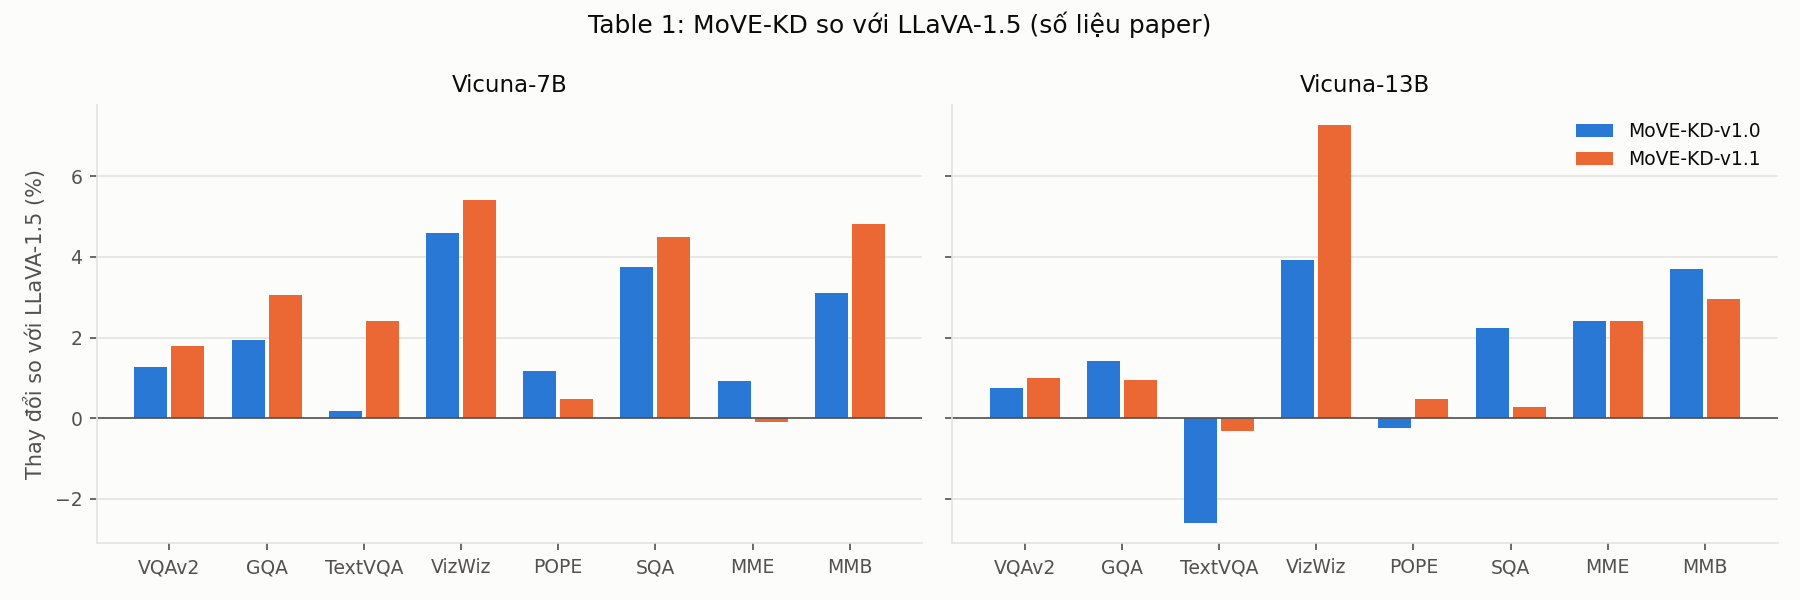
\includegraphics[width=0.9\linewidth]{results_table1.png}
\caption{Mức thay đổi tương đối (\%) của MoVE-KD so với LLaVA-1.5 trên từng benchmark (Table 1).}
\end{figure}

\paragraph{Nhận xét.}
\begin{enumerate}
\item \textbf{Cải thiện ổn định ở 7B.} MoVE-KD-v1.1 tăng trên 7/8 benchmark so với LLaVA-1.5-7B (VizWiz $+2.7$, SQA $+3.0$, MMB $+3.1$); riêng MME giảm nhẹ ($-1.6$).
\item \textbf{7B chưng cất tiệm cận 13B gốc}, thậm chí vượt ở GQA (63.9 so với 63.3) và POPE (86.3 so với 85.9).
\item \textbf{So với RADIO.} RADIO giảm ở VQAv2 ($-2.2$) và TextVQA ($-1.9$), được giải thích là do quên tri thức căn chỉnh ngôn ngữ của CLIP. MoVE-KD không giảm ở hai bộ này nhờ giữ CLIP làm teacher ``neo'' với trọng số 0.8.
\item \textbf{TextVQA là điểm yếu nhất quán} ở 13B và LLaVA-NeXT. Một giải thích bổ sung: không teacher nào trong v1.0/v1.1 chuyên về văn bản, dù repo có hỗ trợ Pix2Struct.
\end{enumerate}

% =====================================================================
\section{Ablation study}

\begin{table}[H]
\centering
\caption{Thêm lần lượt từng thành phần (Table 2 của paper, LLaVA-1.5-7B, teacher v1.0). Avg là trung bình 7 benchmark, không tính MME.}
\label{tab:abl}
\small
\setlength{\tabcolsep}{4.5pt}
\begin{tabular}{@{}lrrrrrrrrr@{}}
\toprule
Phương pháp & VQAv2 & GQA & TextVQA & VizWiz & POPE & SQA & MME & MMB & Avg \\
\midrule
LLaVA-1.5 7B & 78.5 & 62.0 & 58.2 & 50.0 & 85.9 & 66.8 & 1510.7 & 64.3 & 66.5 \\
+ KD (nội suy) & 79.0 & 62.4 & 56.7 & 50.9 & 84.7 & 67.6 & 1507.6 & 62.9 & 66.3 \\
+ Encoder adapter & 79.3 & 62.4 & 57.0 & 51.2 & 85.2 & 68.3 & 1517.8 & 63.8 & 66.7 \\
+ MoLE & 79.1 & 62.8 & 57.3 & 51.9 & 86.4 & 68.7 & 1521.3 & 65.4 & 67.4 \\
+ Token weight & 79.3 & 63.1 & 57.7 & 52.5 & 86.7 & 68.9 & 1524.1 & 66.0 & 67.7 \\
+ Teacher weight & 79.5 & 63.2 & 58.3 & 52.3 & 86.9 & 69.3 & 1524.5 & 66.3 & \best{68.0} \\
\bottomrule
\end{tabular}
\end{table}

\begin{itemize}
\item \textbf{KD ``ngây thơ'' (nội suy) còn tệ hơn không chưng cất} (66.5 $\rightarrow$ 66.3): bằng chứng cho vấn đề bất đồng không gian đặc trưng giữa teacher và student.
\item \textbf{Encoder adapter} ($+0.4$) thay phép nội suy bằng phép chiếu học được, nhờ đó KD bắt đầu có lợi.
\item \textbf{MoLE đóng góp nhiều nhất} ($+0.7$), với POPE $+1.2$ và MMB $+1.6$.
\item \textbf{Token weight} và \textbf{teacher weight} mỗi thành phần thêm $+0.3$. Tổng cộng $+1.5$ Avg, gần một nửa đến từ MoLE.
\end{itemize}

\paragraph{MoLE không KD (Table 3).} Khi bỏ KD, thêm MoLE gần như không đổi kết quả (Avg 64.4 $\rightarrow$ 64.5) dù chỉ thêm khoảng 0,3\% tham số. Như vậy mức tăng ở Bảng~\ref{tab:abl} không đến từ việc thêm tham số mà từ việc MoLE giúp hấp thụ tri thức của teacher.

\paragraph{Trọng số teacher CLIP (Table 4).} Avg lần lượt là 67.1 / 67.5 / \textbf{68.0} / 67.8 với trọng số 0.6 / 0.7 / 0.8 / 0.9. Student khởi tạo từ CLIP và projector cùng LLM đều ``quen'' với không gian đặc trưng của CLIP, nên teacher CLIP cần trọng số lớn; nhưng quá lớn thì giảm phần tri thức học từ các teacher khác.

\paragraph{Đóng băng hay mở băng encoder (Table 5).} Mở băng encoder của LLaVA-1.5 mà không KD làm \textbf{giảm} 5/6 benchmark (POPE $-4.4$, TextVQA $-3.4$, SQA $-2.7$), nên mức tăng của MoVE-KD thực sự đến từ chưng cất chứ không phải từ việc mở băng encoder.

\paragraph{Thêm teacher SAM (v1.0 $\rightarrow$ v1.1).} Thay đổi nhất quán duy nhất là TextVQA tăng ở cả 3 kích thước ($+0.9$ đến $+1.4$); các benchmark khác lên xuống tuỳ kích thước. Khả năng mở rộng theo số teacher vì vậy nên được trình bày như một xu hướng tích cực, chưa phải kết luận chắc chắn.

% =====================================================================
\section{Kết quả tự chạy lại}

\subsection{Môi trường}

1$\times$RTX 3090 24GB (instance vast.ai, ổ 32GB), Python 3.10, torch 2.1.2, transformers 4.37.2. Suy luận fp16, greedy (temperature 0), conv mode \code{vicuna_v1}, batch 1; model 7B chiếm khoảng 15GB VRAM. Để kiểm tra bộ chấm điểm, chúng tôi chấm lại câu trả lời LLaVA-1.5-13B có sẵn trong \code{eval.zip} của LLaVA và thu được POPE 85.95, MME 1531.3, TextVQA 61.25, SQA-IMG 71.64, khớp Table~1 (85.9 / 1531.3 / 61.3 / 71.6). Vì vậy mọi chênh lệch dưới đây đến từ bước chạy model, không phải từ dữ liệu hay script chấm.

\subsection{Tái lập MoVE-KD-v1.1-7B}

\begin{table}[H]
\centering
\caption{Checkpoint \code{jiaojuncao/MoVE-KD-7b-v1.1} chạy lại so với paper.}
\label{tab:repro}
\begin{tabular}{@{}lrrrrr@{}}
\toprule
Benchmark & Số câu & Thời gian & Paper & Tự chạy & Chênh lệch \\
\midrule
POPE (F1 TB) & 8910 & 42 phút & 86.3 & \best{86.06} & $-0.2$ \\
MME (perception) & 2374 & 12 phút & 1509.1 & \best{1510.0} & $+0.9$ \\
TextVQA & 5000 & 35 phút & 59.6 & \best{59.62} & $+0.0$ \\
SQA-IMG & 4241 & 16 phút & 69.8 & \best{69.81} & $+0.0$ \\
\bottomrule
\end{tabular}
\end{table}

POPE F1 theo split là 87.17 / 86.18 / 84.82 (random / popular / adversarial); MME cognition 331.1. Cả 4 benchmark đều lệch không quá 0.2 điểm, riêng MME lệch 0.9 trên thang khoảng 2000. \textbf{Checkpoint công bố đúng là mô hình được báo cáo trong paper.}

\subsection{Baseline LLaVA-1.5-7B trong cùng điều kiện}

Không thể eval LLaVA-1.5 gốc bằng code của repo MoVE-KD: \code{builder.py} nạp mọi model có tên chứa \code{llava} thành \code{EvalMoVELlavaLlamaForCausalLM}, và vì \code{config.json} của LLaVA-1.5 không có khoá \code{moe}, CLIP bị gắn thêm các expert LoRA khởi tạo ngẫu nhiên. Chúng tôi viết \code{scripts/move-kd/eval/baseline.sh} để chạy cùng các wrapper eval nhưng từ một checkout LLaVA gốc.

\begin{table}[H]
\centering
\caption{Baseline tự chạy so với paper, và mức tăng của MoVE-KD so với từng baseline.}
\label{tab:baseline}
\small
\begin{tabular}{@{}lrrrrr@{}}
\toprule
 & \multicolumn{2}{c}{LLaVA-1.5-7B} & MoVE-KD-v1.1 & \multicolumn{2}{c}{MoVE-KD $-$ baseline} \\
\cmidrule(lr){2-3}\cmidrule(lr){5-6}
Benchmark & Paper & Tự chạy & Tự chạy & so với tự chạy & so với paper \\
\midrule
POPE (F1 TB) & 85.9 & 85.92 & 86.06 & $+0.1$ & $+0.4$ \\
MME (perception) & 1510.7 & 1504.6 & 1510.0 & $+5.4$ & $-0.7$ \\
TextVQA & 58.2 & 58.23 & 59.62 & $+1.4$ & $+1.4$ \\
SQA-IMG & 66.8 & \textcolor{red!70!black}{\textbf{69.46}} & 69.81 & $+0.4$ & $+3.0$ \\
\bottomrule
\end{tabular}
\end{table}

\begin{figure}[H]
\centering
\begin{subfigure}{0.49\linewidth}
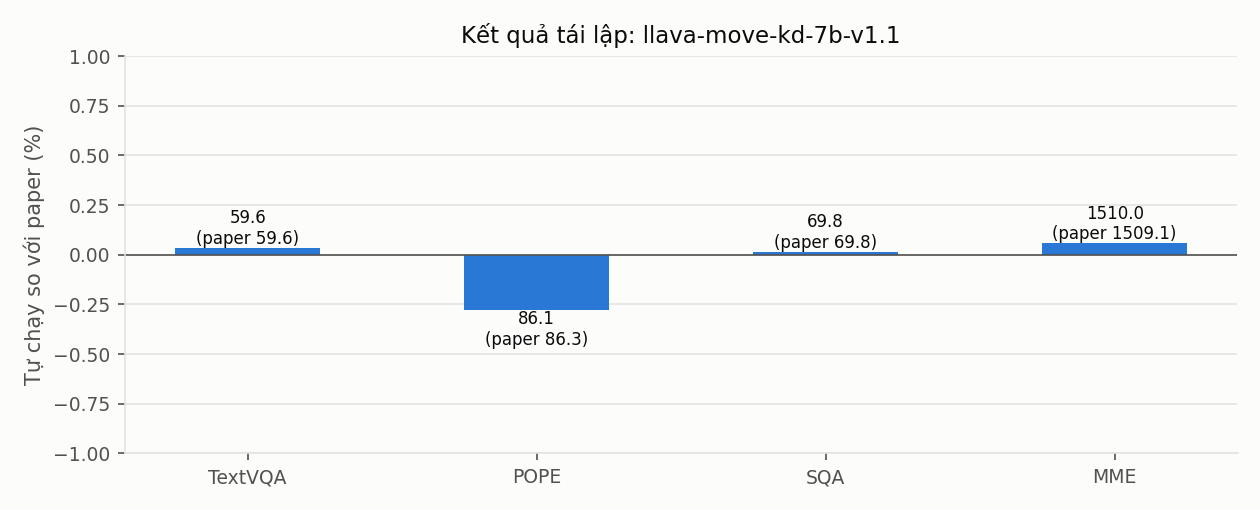
\includegraphics[width=\linewidth]{results_reproduced_llava-move-kd-7b-v1.1.png}
\caption{MoVE-KD-v1.1-7B}
\end{subfigure}\hfill
\begin{subfigure}{0.49\linewidth}
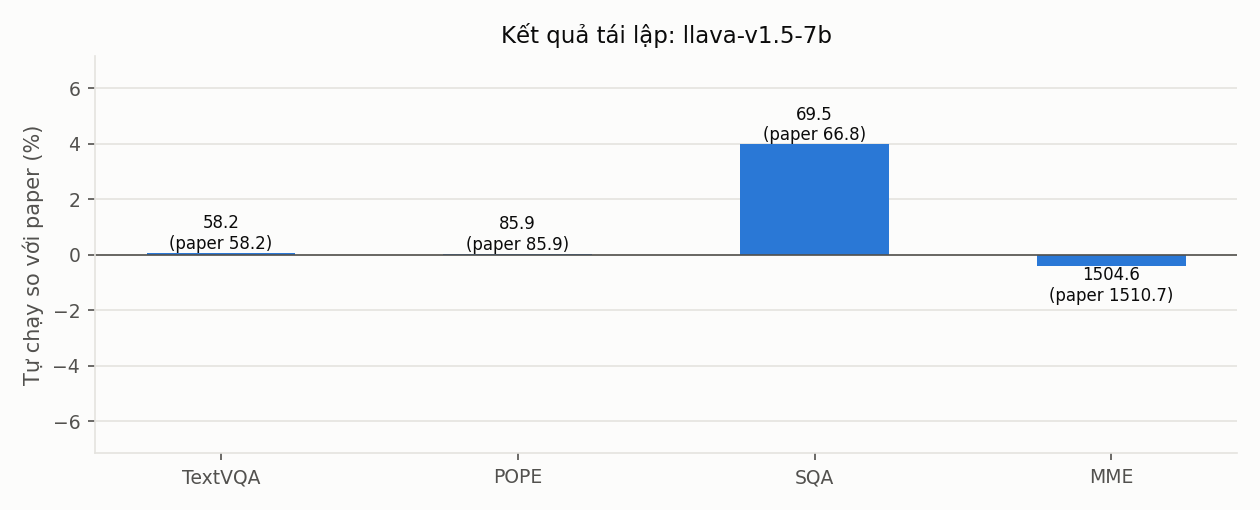
\includegraphics[width=\linewidth]{results_reproduced_llava-v1.5-7b.png}
\caption{LLaVA-1.5-7B}
\end{subfigure}
\caption{Chênh lệch giữa kết quả tự chạy và số liệu paper.}
\end{figure}

\paragraph{Nhận xét.}
\begin{enumerate}
\item \textbf{Baseline khớp paper ở 3/4 benchmark}: TextVQA và POPE trùng tới 0.1, MME lệch $-6.1$ (dưới 0,5\% thang điểm).
\item \textbf{SQA là ngoại lệ}: baseline tự chạy đạt 69.46, cao hơn con số 66.8 paper dùng tới 2.7 điểm. Bộ chấm đã được kiểm chứng, nên chênh lệch nằm ở bước sinh câu trả lời. Một khả năng là 66.8 được đo bằng phiên bản code hoặc prompt cũ hơn; chúng tôi chưa kiểm chứng giả thuyết này.
\item \textbf{Hệ quả cho kết luận của paper.} So với baseline cùng điều kiện, MoVE-KD vẫn tăng ở cả 4 benchmark, nhưng mức tăng SQA giảm từ $+3.0$ xuống \textbf{$+0.4$}. Mức tăng rõ nhất còn lại là TextVQA ($+1.4$), phù hợp với lập luận rằng các teacher (EVA-02, ConvNeXt độ phân giải cao, SAM) bổ sung chi tiết cục bộ và chữ. POPE ($+0.1$) và MME ($+5.4$) chỉ tăng nhẹ, ở mức dao động khi chạy lại.
\end{enumerate}

% =====================================================================
\section{Trực quan hoá [CLS] attention và routing MoLE}

Repo gốc không có code vẽ Fig~5 của paper, nên chúng tôi viết \code{scripts/move-kd/visualize_attention.py}. Script tính [CLS] attention giống hệt cách tính token weight trong \code{forward()}: lấy attention ở layer $-2$, trung bình theo head, hàng [CLS], qua softmax rồi đưa về lưới $24\times24$. Script chỉ nạp vision encoder (shard thứ 3 của checkpoint) nên chạy được trên CPU, và vẽ thêm bản đồ expert MoLE được chọn cho từng patch.

\begin{figure}[H]
\centering
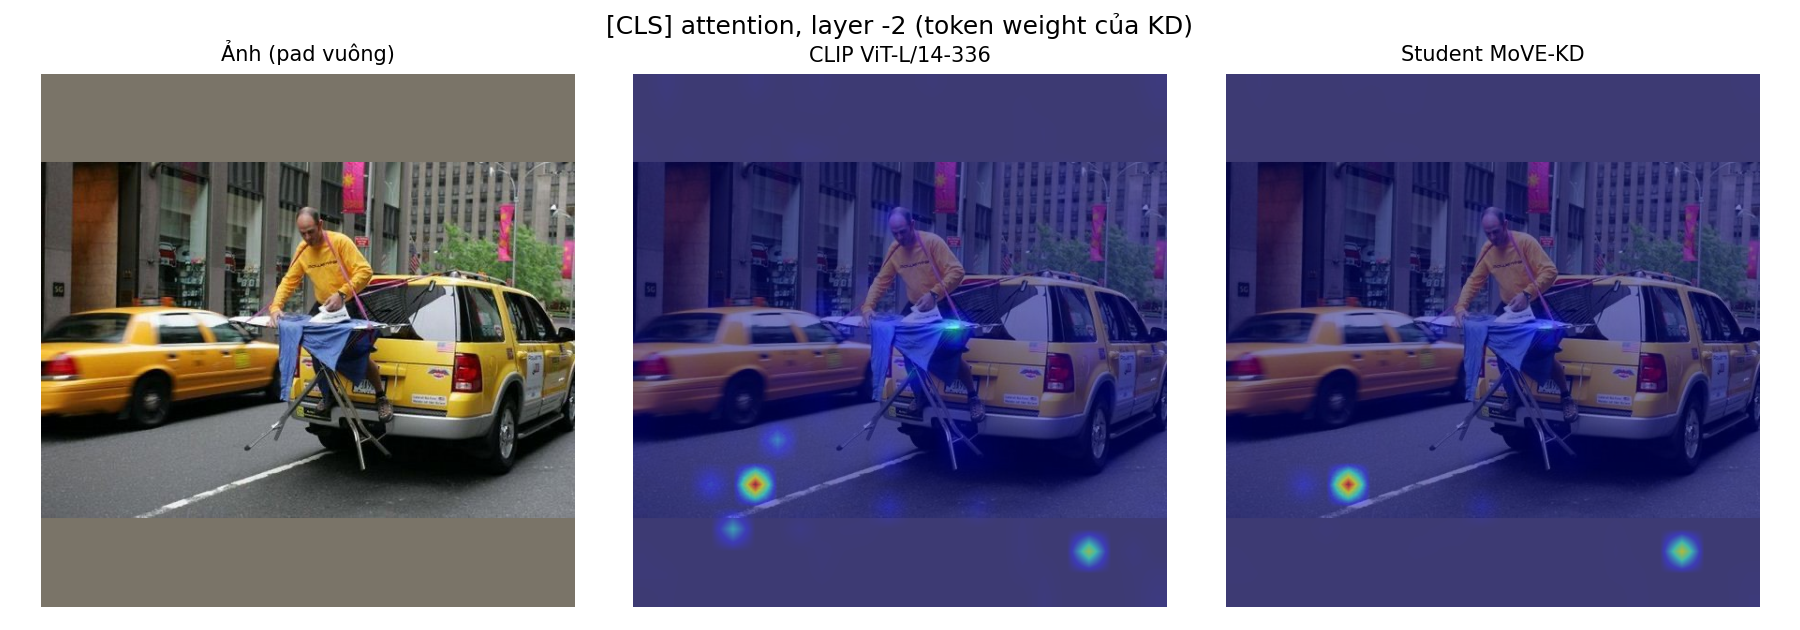
\includegraphics[width=\linewidth]{attn_extreme_ironing.png}\\[4pt]
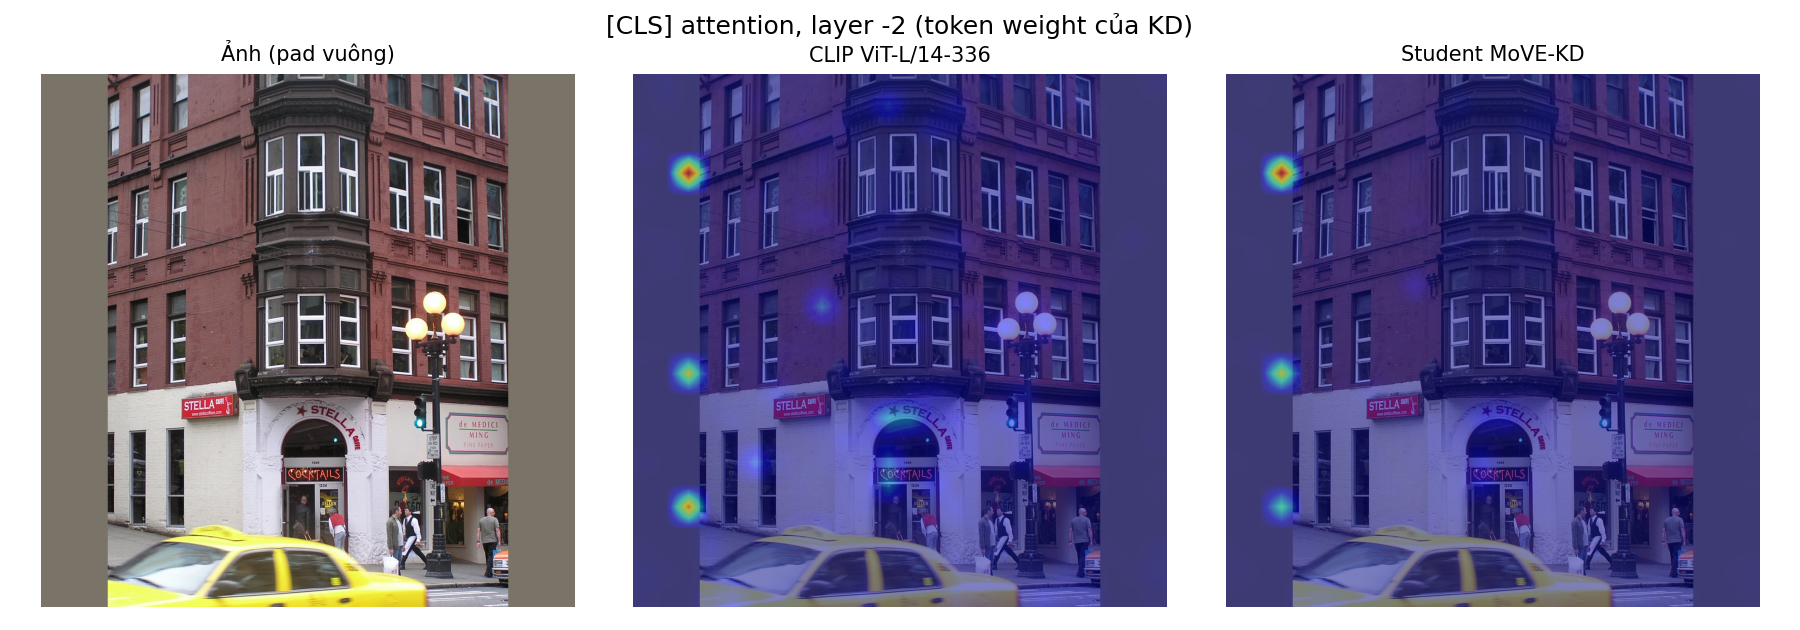
\includegraphics[width=\linewidth]{attn_0004c9478eeda995.png}
\caption{Ảnh gốc / [CLS] attention của CLIP gốc / của student MoVE-KD-v1.1 (ảnh mẫu LLaVA và ảnh TextVQA).}
\label{fig:attn}
\end{figure}

\begin{figure}[H]
\centering
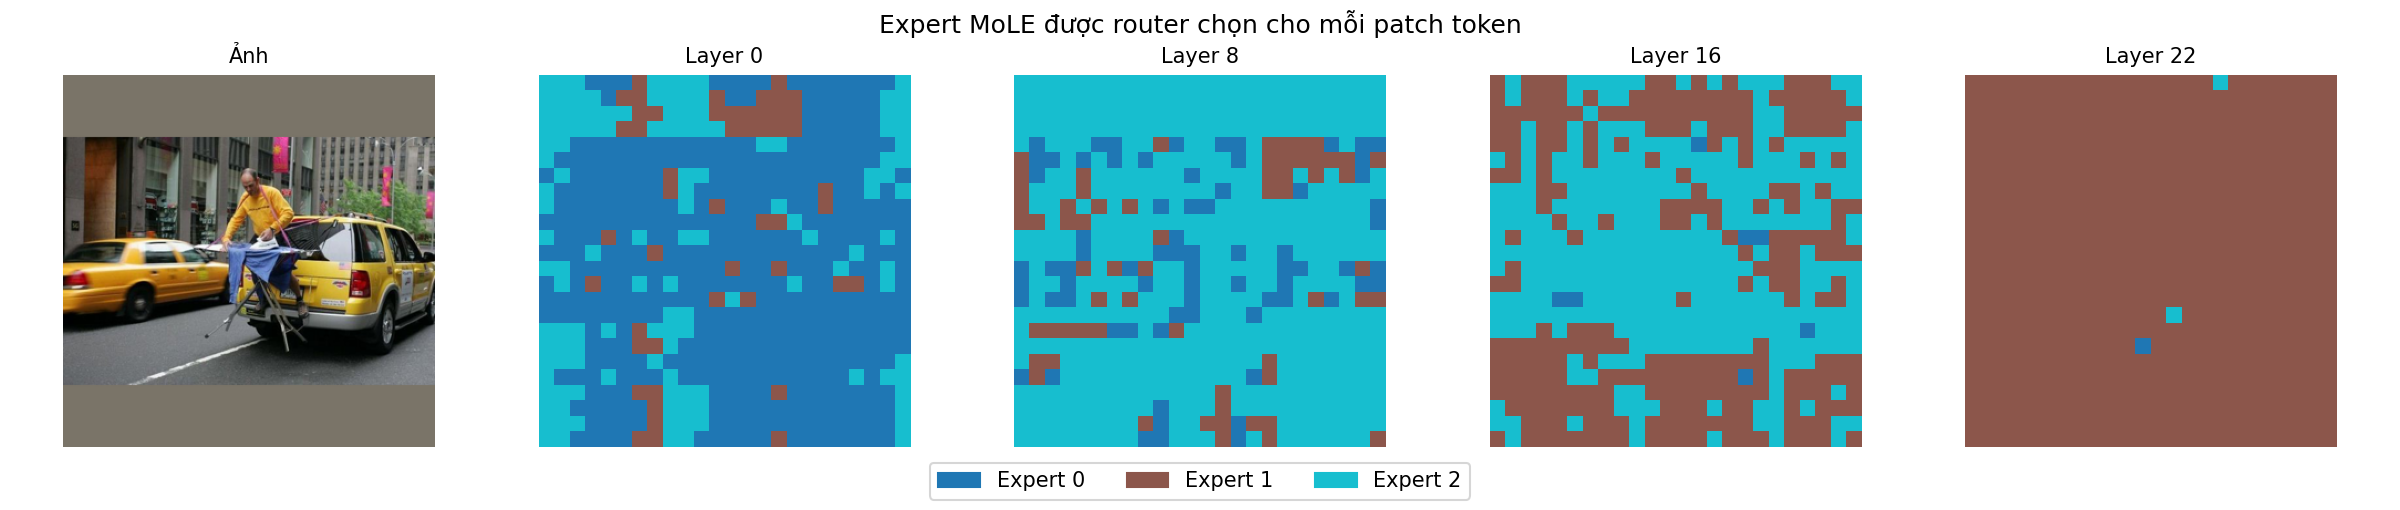
\includegraphics[width=\linewidth]{routing_extreme_ironing.png}\\[4pt]
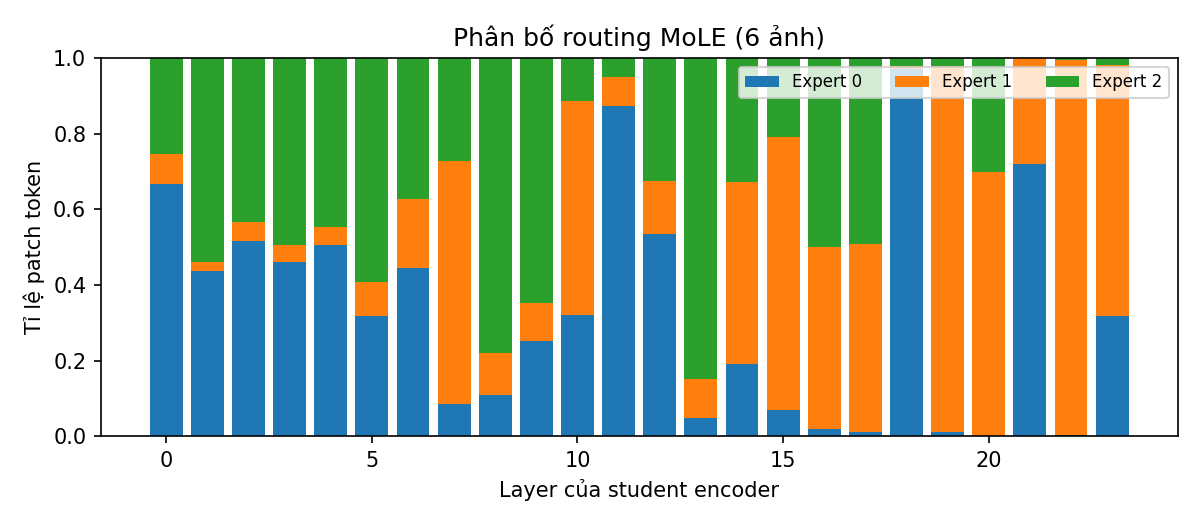
\includegraphics[width=0.62\linewidth]{routing_share.png}
\caption{Trên: expert MoLE được chọn cho mỗi patch tại layer 0, 8, 16, 22. Dưới: tỉ lệ patch token vào từng expert theo layer.}
\label{fig:routing}
\end{figure}

\begin{itemize}
\item \textbf{Attention dồn vào vài token đơn lẻ.} Ở cả CLIP lẫn student, [CLS] attention tập trung vào vài token ở vùng nền hoặc dải padding (do \code{expand2square}), không nằm trên vật thể chính. Đây là các token ``artifact'' có norm cao \cite{registers}. Hệ quả là token weight trong KD thực chất chỉ tập trung vào vài vị trí.
\item \textbf{Student gần như giữ nguyên bản đồ của CLIP} ở cả 6 ảnh thử, chỉ bỏ bớt vài đỉnh phụ. Chúng tôi \emph{không thấy rõ} hiện tượng như Fig~5 của paper (student chuyển hẳn attention từ nền sang vật thể hay chữ).
\item \textbf{Routing MoLE chuyên hoá theo layer hơn là theo nội dung.} Ở layer 0--6, token chia khá đều giữa 3 expert; từ khoảng layer 10, một expert chiếm 70--100\% token. Điều này khớp với một đặc điểm của code: ở chế độ sparse, router chỉ nhận gradient từ balance loss nên dễ suy biến về một expert ở từng layer. MoLE ở đây hoạt động gần với ``mỗi layer một LoRA'' hơn là ``mỗi token một expert''.
\end{itemize}

% =====================================================================
\section{Chạy thử pipeline huấn luyện}

\subsection{Smoke-test Stage 1}

Huấn luyện đầy đủ cần khoảng 8$\times$A100 nên không khả thi. Để kiểm tra code huấn luyện, chúng tôi chạy \code{scripts/move-kd/smoke_pretrain.sh}: Stage~1 với đủ 4 teacher (CLIP, SAM, EVA-02, ConvNeXt), MoLE 3 expert và encoder adapter, nhưng thay Vicuna-7B bằng TinyLlama-1.1B, dùng 100 mẫu LCS-558K, 30 bước, batch 2.

\begin{itemize}
\item Chạy hết 30 bước trong 2 phút trên RTX 3090, VRAM đỉnh 17.8GB.
\item Tạo đủ 3 file \code{mm_projector.bin}, \code{mole_encoder.bin}, \code{encoder_adapter.bin}.
\item Loss tổng giảm từ 10.13 (bước 1) xuống 4.68 (bước 30); trung bình 5 bước đầu là 8.0, 5 bước cuối là 4.5. Đường loss dao động mạnh vì batch chỉ có 2 mẫu.
\end{itemize}

\subsection{Bug trong code huấn luyện}

Lần chạy đầu bị lỗi ngay bước 1 với thông báo \code{Tensors must have same number of dimensions: got 2 and 1}. In shape từng bước cho thấy vision tower nhận $(2, 3, 336, 336)$ nhưng trả về $(576, 1024)$, tức mất chiều batch. Nguyên nhân:

\begin{itemize}
\item Khi huấn luyện, vision tower được dựng bằng \code{build_vision_tower(model_args)}. \code{ModelArguments} không có trường \code{kd}, nên \code{CLIPVisionTower.forward} chỉ trả về tensor features.
\item \code{encode_images} trong \code{llava_arch.py} luôn unpack 2 giá trị, nên Python tách tensor theo chiều batch: ảnh 1 thành \code{image_features}, ảnh 2 thành \code{image_forward_outs}. Với batch khác 2, lỗi unpack xảy ra ngay.
\item Lúc eval không gặp lỗi này vì tower được dựng từ \code{config}, vốn có \code{config.kd}.
\end{itemize}

Cách sửa là thêm một dòng trong \code{initialize_teachers} (\code{move_llava_llama.py}) để đồng bộ \code{config.kd} sang vision tower:

\begin{lstlisting}[language=Python]
self.config.kd['kd_mode'] = self.training_args.kd
self.get_model().get_vision_tower().args.kd = self.config.kd
\end{lstlisting}

Bug này ảnh hưởng cả Stage~1 lẫn Stage~2, vì cả hai đều dựng tower từ \code{model_args}.

% =====================================================================
\section{Ghi chú tái lập}

\begin{enumerate}
\item \textbf{Tên checkpoint phải chứa \code{llava}}, nếu không \code{builder.py} nạp model như LLM thuần và \code{image_processor = None}. \code{download_ckpt.sh} tải về \code{checkpoints/llava-move-kd-7b-v1.1}.
\item \textbf{Phiên bản thư viện.} Cần \code{timm>=0.9} cho teacher ConvNeXt (dù \code{pyproject.toml} pin 0.6.13), \code{peft==0.10.0}, \code{numpy<2}, \code{transformers==4.37.2} và \code{setuptools<70} để build \code{flash-attn==2.5.8}. Các file \code{scripts/zero2*.json} bị \code{.gitignore} bỏ qua nên phải sinh bằng \code{setup.sh}.
\item \textbf{Teacher hardcode bf16 và đường dẫn} \code{./checkpoints/...}, nên huấn luyện cần GPU Ampere trở lên và phải chạy từ thư mục gốc repo.
\item \textbf{Log nạp model có khoảng 390 cảnh báo} \code{copying from a non-meta parameter}: vô hại, vì trọng số thật được nạp sau đó, như kết quả Bảng~\ref{tab:repro} xác nhận.
\item \textbf{Ổ đĩa nhỏ (32GB).} Dùng \code{remotezip} để chỉ lấy đúng 500 ảnh POPE và 3166 ảnh TextVQA thay vì tải nguyên các file zip 6--7GB.
\end{enumerate}

Toàn bộ lệnh tái lập nằm ở mục 2.7 của \code{Experiments.md}; trên Colab A100 có thể dùng \code{notebooks/move_kd_colab.ipynb}.

% =====================================================================
\section{Kết luận}

\begin{enumerate}
\item Checkpoint MoVE-KD-v1.1-7B công bố tái lập đúng số liệu paper trên POPE, MME, TextVQA và SQA (lệch $\le 0.2$ điểm).
\item So với baseline LLaVA-1.5-7B chạy cùng điều kiện, MoVE-KD tăng ở cả 4 benchmark nhưng nhỏ hơn mức paper báo cáo; mức tăng SQA giảm từ $+3.0$ xuống $+0.4$, rõ nhất còn lại là TextVQA $+1.4$.
\item Student kế thừa phần lớn [CLS] attention của CLIP; routing của MoLE suy biến theo layer thay vì chuyên hoá theo nội dung.
\item Pipeline huấn luyện với đủ 4 teacher chạy được trên một GPU 24GB sau khi sửa một bug có sẵn trong code.
\end{enumerate}

\paragraph{Hướng tiếp theo.} Kiểm chứng nguồn gốc con số SQA 66.8 của baseline; thử chế độ dense MoLE để xem routing có còn suy biến; và nếu có tài nguyên, chạy ablation với baseline tự chạy thay vì số trong paper.

% =====================================================================
\begin{thebibliography}{99}\small
\bibitem{movekd} J. Cao et al. MoVE-KD: Knowledge Distillation for VLMs with Mixture of Visual Encoders. CVPR 2025. arXiv:2501.01709.
\bibitem{llava} H. Liu et al. Visual Instruction Tuning. NeurIPS 2023; Improved Baselines with Visual Instruction Tuning. CVPR 2024.
\bibitem{flamingo} J.-B. Alayrac et al. Flamingo: a Visual Language Model for Few-Shot Learning. NeurIPS 2022.
\bibitem{blip2} J. Li et al. BLIP-2. ICML 2023; W. Dai et al. InstructBLIP. NeurIPS 2023.
\bibitem{qwenvl} J. Bai et al. Qwen-VL: A Frontier Large Vision-Language Model with Versatile Abilities. 2023.
\bibitem{minigemini} Y. Li et al. Mini-Gemini: Mining the Potential of Multi-modality Vision Language Models. 2024.
\bibitem{s2} B. Shi et al. When Do We Not Need Larger Vision Models? ECCV 2024.
\bibitem{eagle} M. Shi et al. Eagle: Exploring the Design Space for Multimodal LLMs with Mixture of Encoders. 2024.
\bibitem{cambrian} S. Tong et al. Cambrian-1: A Fully Open, Vision-Centric Exploration of Multimodal LLMs. 2024.
\bibitem{sphinx} Z. Lin et al. SPHINX: The Joint Mixing of Weights, Tasks, and Visual Embeddings for Multi-modal LLMs. 2023.
\bibitem{hinton} G. Hinton, O. Vinyals, J. Dean. Distilling the Knowledge in a Neural Network. 2015.
\bibitem{fitnets} A. Romero et al. FitNets: Hints for Thin Deep Nets. ICLR 2015.
\bibitem{dinov2} M. Oquab et al. DINOv2: Learning Robust Visual Features without Supervision. 2023.
\bibitem{fd} Y. Wei et al. Contrastive Learning Rivals Masked Image Modeling in Fine-tuning via Feature Distillation. 2022.
\bibitem{radio} M. Ranzinger et al. AM-RADIO: Agglomerative Vision Foundation Model -- Reduce All Domains Into One. CVPR 2024.
\bibitem{theia} J. Shang et al. Theia. 2024; M. B. Sariyildiz et al. UNIC. ECCV 2024.
\bibitem{multiteacher} S. You et al. Learning from Multiple Teacher Networks. KDD 2017.
\bibitem{ones} F. Xue et al. One Student Knows All Experts Know: From Sparse to Dense. 2022.
\bibitem{llavamod} F. Shu et al. LLaVA-MoD: Making LLaVA Tiny via MoE Knowledge Distillation. 2024.
\bibitem{mdrt} T. Huang et al. Masked Distillation with Receptive Tokens. ICLR 2023.
\bibitem{registers} T. Darcet et al. Vision Transformers Need Registers. ICLR 2024.
\bibitem{moe} R. A. Jacobs et al. Adaptive Mixtures of Local Experts. 1991; W. Fedus et al. Switch Transformers. JMLR 2022.
\bibitem{moellava} B. Lin et al. MoE-LLaVA. 2024; Y. Li et al. Uni-MoE. 2024.
\bibitem{lora} E. J. Hu et al. LoRA: Low-Rank Adaptation of Large Language Models. ICLR 2022.
\bibitem{mole} S. Dou et al. LoRAMoE. 2023; X. Wu et al. Mixture of LoRA Experts. ICLR 2024.
\end{thebibliography}

\end{document}
